\documentclass[11pt,twoside,a4paper]{report}

\usepackage[english]{babel}
\usepackage[utf8]{inputenc}
\usepackage{amsmath}
\usepackage{hyperref}
\usepackage{color,soul}
\usepackage{graphicx}
\newcommand\Colorhref[3][blue]{\href{#2}{\small\color{#1}#3}}
\usepackage[colorinlistoftodos]{todonotes}
\usepackage[letterpaper, margin=1in]{geometry}
\usepackage[boxruled,lined]{algorithm2e}
\usepackage{array}
\newcolumntype{x}[1]{>{\centering\arraybackslash\hspace{0pt}}p{#1}}

% \title{\textbf{Online Segmentation for Multivariate Sequential Data}}

% \author{Ilaria Lauzana}

% \date{\today}

\newpage
\begin{document}

% \maketitle

\begin{titlepage}
\begin{center}

\includegraphics[width=.3\textwidth]{EPFL-Logo.jpg}\\[5pt]
 \vspace{2cm}
\textsc{Master 2 - Semester Project} \\
 \vspace{2cm}
 {\huge\bfseries Online Segmentation for Multivariate Sequential Data \\}
 \vspace{1.5cm}
 {\Large Ilaria Lauzana}\\[5pt]
 ilaria.lauzana@epfl.ch\\[14pt]
 \vspace{2cm}
{\large \bfseries Supervised by} \\[5pt]
{\large Nadia Figueroa}\\[5pt]
{\large Jos\'e Medina}\\[5pt]
{\large Prof. Aude Billard}\\[5pt]
\vfill
\today
\end{center}
\end{titlepage}

\clearpage

\tableofcontents

\newpage

\chapter{Introduction} \label{ch:intro}

Machine learning algorithms have many applications and have to deal with different types of datasets. When considering techniques for robotics applications requiring demonstration examples, datasets are often represented by a sequence of data points sampled at a specific frequency, called time series.

However, time series generally include multiple sequential tasks which are independent from one another and should be modeled separately, such as in the example of a carrot grating task demonstration depicted in Figure \ref{fig:initial}.

\begin{figure}[h]
\centering
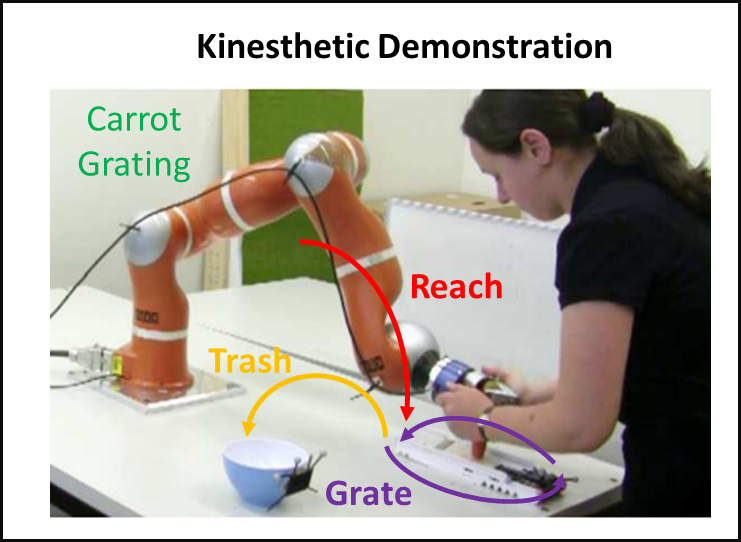
\includegraphics[width=.65\textwidth]{carrot_grating.png}
\caption{Kinesthetic demonstration of a carrot grating task.}
\label{fig:initial}
\end{figure}

For this reason, many algorithms are available to partition data points into segments and are referred to as \textit{segmentation algorithms}. Most successful methods, though, require offline processing and need for the data to be given in batch (see \cite{lucia} and \cite{nadia} for an extensive review).

However, scenarios where we need to extract models from an incoming stream of data prevent the application of segmentation algorithms in an offline fashion. Moreover, this creates a bottleneck in the learning pipeline.

Motivated by this, we present an \textit{online} segmentation algorithm which allows to enable online learning.

\section{Online segmentation}

The statistical and machine learning community has mostly tackled the online segmentation problem as a problem of \textit{changepoint detection}, with the \textit{changepoint} being a temporal location where a change occurs in the underlying properties of the data. More precisely, assuming that the segments are modeled with a certain parametric function, a changepoint is the location where the model's parameters vary, thus defining the end of the previous segment and the beginning of a new one. This may be viewed in Figure \ref{fig:timeseries}, with a univariate time series modeled with Gaussian functions whose parameters vary at the changepoints, highlighted with red lines.

\begin{figure}[h]
\centering
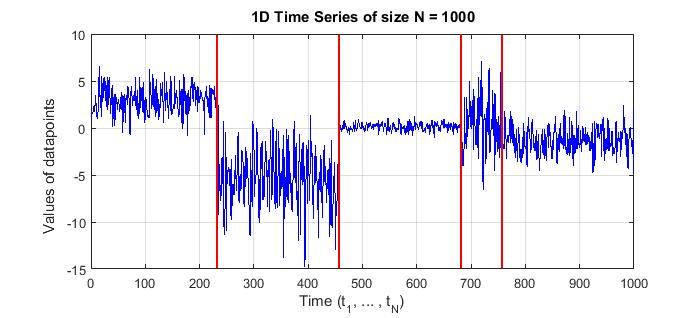
\includegraphics[width=.9\textwidth]{1d_series_1000_segments.jpg}
\caption{Example of a univariate time series with 1000 datapoints. Changepoints are shown in red and delimit 5 segments.}
\label{fig:timeseries}
\end{figure}

Available algorithms for changepoint detection as in \cite{adams}, \cite{fearn1}, \cite{fearn2} and \cite{champ} all share a similar strategy: in order to correctly detect when a changepoint has occurred (represented by a state $s_t$), the time series is processed during sampling to predict whether the current data point fits the model's parameters $\theta$. To make this prediction, Bayesian inference is used, requiring two types of priors probability functions: the first is a prior on the segment's parameters, while the second is a prior on the length of the segments.

The prior on the segment's parameters represents the belief that the observations are generated from a model with parameters $\theta$ which can be drawn from this distribution. Using this prior distribution it is possible to find the posterior predictive distribution for a new observation $\tilde{x}$, given the data $x_{1:t}$ and the parameters $\eta$ of the prior, as:

\begin{equation} \label{eq:priorPar}
P(\tilde{x} | x_{1:t}, \eta) = \int P(\tilde{x} | \theta, \eta) P(\theta | x_{1:t}, \eta) d\theta .
\end{equation}

It may be assumed to be \textit{conjugate} to the model $P(\tilde{x} | \theta, \eta)$, as in \cite{adams}, \cite{fearn1} and \cite{fearn2}. In these cases, the predictive posterior probability for the new datum can be found analytically and has the same form of the prior.
In the case of \cite{champ} instead, the model is approximated by using the Bayesian Information Criterion (BIC), thus no conjugate prior is needed. On the other hand, the simplification is made at the expense of larger uncertainties.

Secondly, in all the algorithms the prior on the segment length represents the probability of finding a changepoint at a certain distance with respect to the previous one. It is used to calculate the posterior probabilities for the current state $s_t$, which represents the eventual presence of a changepoint, given the data $x_{1:t}$ sampled up to the current time step and the previous state $s_{t-1}$, by following Bayes' rule. The posterior is then given by:

\begin{equation} \label{eq:post}
\underbrace{P(s_t | x_{1:t}, s_{t-1})}_{\text{\shortstack{Posterior \\ Probability}}} = \frac{\overbrace{P(s_{t-1} | x_{1:t-1}, s_{t-2})}^{\text{\shortstack{Previous step's \\Posterior Probability}}}\overbrace{P(x_t | x_{1:t}, \eta)}^{\text{\shortstack{Posterior Predictive\\(Model Likelihood)}}}  \overbrace{P(s_t | s_{t - 1})}^{\text{\shortstack{Prior on\\segment length}}}}{  \underbrace{P (x_{1:t}) }_{\text{\shortstack{Model \\ Evidence}}}}
\end{equation}

Finally, the algorithms mentioned above differ regarding to the computational cost. In fact, while \cite{adams} and \cite{fearn1} are exact inference algorithms and for each step $t$ require $O(t)$ computations, \cite{fearn2} and \cite{champ} approximate the algorithm in \cite{fearn1} by reducing the number of data points considered in the calculation of the probabilities, thus reducing also the computation time to a constant for each time step.

Unfortunately, all these algorithms deal only with univariate data, while most of the time series used in robotics applications are multidimensional.

\section{Proposed Approach}
After evaluating the online univariate algorithms presented in \cite{adams}-\cite{champ}, we decided to propose a multivariate algorithm that is built upon the one presented by Adams and MacKay \cite{adams}, because a multivariate online segmentation technique would allow to speed up online learning in robotics.

The algorithm was chosen because it is a basis for similar algorithms as the ones in \cite{fearn1}-\cite{champ} and because it has been proven quite powerful. Its expansion to multivariate time series is described in \ref{sec:bayes} and it consists in a change of the form of the prior probability over the model's parameters, and in consequence the form of the posterior probability.

On the other hand, the algorithm is very computationally intensive and for each iteration $t$ require $O(t)$ computations, as already discussed. Moreover, considering a multivariate time series the update of the parameters of the predictive posterior probability also require a longer time because it now deals with matrices multiplication, and computations also increase with the number of dimensions. Therefore, due to computational constraints, we have explored approximations techniques as the ones found in \cite{fearn2} and \cite{champ}. The chosen method for approximation is presented in section \ref{sec:impl}.

Finally, we evaluate our approach in both simulations and real data from demonstrations of sequential tasks, as discussed in Chapter \ref{ch:exp}.


\newpage

\chapter{Bayesian Online Changepoint Detection Algorithm}

The algorithm presented by Adams and MacKay and reported in \cite{adams}, tries to solve the changepoint detection problem by using a Bayesian approach in order to find the current "run length" $r_t$, which represents the time since the last changepoint. Storing the run length found for all time steps, it is then possible to retrace back the previous positions of the changepoints. 

The algorithm uses equation \ref{eq:post} and it basically combines:
\begin{enumerate}
\item the prior distribution representing the belief about the segment length;
\item the predictive probabilities of a new datum for each possible run length;
\item the posterior distribution of the run length calculated at the previous time step.
\end{enumerate}

The prior distribution of the segment length represents the prior belief of the distance between two changepoints. In the algorithm by Adams and Mackay, this prior is represented by a $hazard$ $function$ $H(r_t)$ equal to a Geometric distribution with fixed parameter $\lambda$, such that the function $H(r_t) = 1/\lambda$ represents the assumption of a constant rate of changepoints. It is then a uninformative prior which is useful not to bias the results in cases when a priori knowledge is limited.

The posterior predictive probabilities of a new datum are calculated by assuming a prior distribution on the parameters of the model. A $conjugate$ $prior$ for the likelihood of the model is used, allowing to calculate the posterior distribution in analytic form and with the same parametric form as the prior distribution. With this assumption, the posterior predictive distribution may be directly built by updating correctly the prior's parameters, without the need of performing any integration as instead was done in equation \ref{eq:priorPar}, and can be computed in closed form.

The algorithm also takes into account the posterior distribution calculated at the previous time step, thus allowing for a recursion without the need to repeat previous calculations at each step. The initial condition of the posterior distribution considers the presence of a changepoint right before the beginning of our inference; in this way, the first datapoint's run length will necessarily be 1.

The original algorithm deals with univariate time series represented by Normal distributions with unknown mean and/or unknown variance, to whose models correspond different conjugate priors and thus different forms of the predictive probabilities. Here, we consider the case of univariate Normal distributions with unknown mean and variance was considered and we extend the approach to the multivariate case with unknown mean and covariance matrix. The univariate case and the multivariate case are discussed in details in the next sections in order to explain the algorithm and to show how the derivation to the multidimensional case was performed.

\section{Univariate Gaussian with Unknown Mean and Variance}

\paragraph{Conjugate Prior on Model Parameters.}

In the case of unidimensional data sampled by a Gaussian $N(\mu,\sigma^2)$ with both mean and variance changing at changepoints, the conjugate prior to the model is the Normal-Inverse-Gamma (NIG) distribution. Following \cite{book1} and \cite{book2}, this distribution is a combination of a Normal prior on the mean $\mu$ and an Inverse Gamma prior distribution on the variance $\sigma^2$:
\begin{equation}
NIG(\mu, \sigma^2 | \mu_0, \kappa_0, \alpha_0, \beta_0) = N(\mu | \mu_0, \kappa_0\sigma^2)Gamma^{-1}(\sigma^2 | \alpha_0, \beta_0),
\end{equation}
where $\mu_0$ is the prior's mean, $\kappa_0$ is a multiplication constant for the variance and $\alpha_0$ and $\beta_0$ are parameters of the Inverse Gamma. It follows that the posterior predictive distribution will also be a NIG distribution, having:
\begin{equation}
\tilde{x} | X, \mu, \sigma^2  \sim NIG(\mu, \sigma^2 | \mu_n, \kappa_n, \alpha_n, \beta_n),
\end{equation}
and whose parameters can directly be derived by the parameters of the prior to get:
\begin{equation}
\mu_n = \frac{\kappa_0\mu_0 + n\bar{x}}{\kappa_0 + n},
\end{equation}
\begin{equation}
\kappa_n = \kappa_0 + n,
\end{equation}
\begin{equation}
\alpha_n = \alpha_0 + n/2,
\end{equation}
\begin{equation}
\beta_n = \beta_0 + \frac{1}{2} \sum_{i=1}^{n} (x_i - \bar{x})^2 + \frac{\kappa_0n(\bar{x} - \mu_0)^2}{2(\kappa_0 + n)}.
\end{equation}

These parameters are updated after each iteration of the algorithm considering the new sampled observation, thus after only a few steps they are representative of the model and it is possible to quickly determine when they have changed. Moreover, the algorithm is not very sensitive to hyperparameters.

\paragraph{Prior on Segment Length.}

As already introduced in the previous section, the other prior distribution that is defined is a distribution on the segment length, represented in this case by the hazard function $H(r_t)$, a geometric distribution with constant rate given by $\lambda$. Thus, the prior is given by: $P(r_t | r_{t - 1}) = H(r_t) = \frac{1}{\lambda}$.

\paragraph{Detection Algorithm.}

After the initialization of prior's parameters $\mu_0$, $\kappa_0$, $\alpha_0$ and $\beta_0$, the algorithm then proceeds by iterating over the whole time series. So, for t ranging from 1 to N, the number of datapoints, it performs:
 
\begin{enumerate}

\item Calculation of the posterior predictive probability for the new datum $x_t$:
\begin{equation}\label{eq:first}
P(x_t | \mu^{(r_t)}, (\sigma^2)^{(r_t)}) = NIG(\mu^{(r_t)}, (\sigma^2)^{(r_t)} | \mu_t, \kappa_t, \alpha_t, \beta_t),
\end{equation} 
giving a measure for the likelihood of the new datum to be generated by the parameters associated to each possible run length.

\item Calculation of joint probabilities for the run length $r_t$ and the data from 1 up to t, $x_{1:t}$. There are two different types; the $growth$ probabilities represent the probabilities for the new datum to be part of the current segment and thus to increase the previous step's run length by one. Therefore, the probability for each possible run length j is given by the probability of having a run length of j-1 in the previous time step, combined with the predictive distribution of the current observation and the prior on the segment length:
\begin{equation}\label{eq:second1}
P(r_t = j , x_{1:t}) = P(r_{t-1} , x_{1:(t-1)})  P(x_t | \mu^{(r_t)}, (\sigma^2)^{(r_t)})  P(r_t | r_{t - 1}),
\end{equation}
with the prior on the segment length being in this case:
\begin{equation}
P(r_t | r_{t - 1}) = (1-H(r_t)).
\end{equation}
The $changepoint$ probability, instead, is the probability of the presence of a changepoint at the current time step, such that the run length $r_t = 0$. This happens independently on the value of the run length at the previous time step, thus in this case the probability is given by the sum of all the joint probabilities calculated in the previous time step, combined with the current observation's predictive distribution and the prior on segment length:
\begin{equation}
P(r_t = 0 , x_{1:t}) = \sum_{j=0}^{t-1} P(r_{t-1} = j , x_{1:(t-1)})  P(x_t | \mu^{(r_t)}, (\sigma^2)^{(r_t)})  P(r_t | r_{t - 1}),
\end{equation}
with the prior on segment length being:
\begin{equation}\label{eq:second4}
P(r_t | r_{t - 1}) = H(r_t).
\end{equation} 
The prior on the segment length is different for the two joint distributions as in the case of the changepoint probability we are interested in the probability of a changepoint to happen, which is given by the hazard function $H(r_t)$, while in the case of the growth probability we take $1 - (H(r_t))$ as we are interested in the probability of no changepoint occurring.

\item Calculation of the posterior distribution from the previously calculated joint distributions for each possible run length:
\begin{equation}\label{eq:third1}
P(r_t | x_{1:t}) = \frac{P(r_t , x_{1:t})} {P(x_{1:t})},
\end{equation} 
thus normalizing the joint distribution over the model evidence given by:
\begin{equation}\label{eq:third2}
P(x_{1:t}) = \sum_{j=0}^{t} P(r_t = j , x_{1:t}).
\end{equation} 

\item Update of the model parameters to be used in the next iteration:
\begin{equation}\label{eq:fourth1}
\mu_{t+1} = \frac{\kappa_0\mu_0 + t\bar{x}}{\kappa_0 + t}, 
\end{equation} 
\begin{equation}
\kappa_{t+1} = \kappa_0 + t,
\end{equation}
\begin{equation}
\alpha_{t+1} = \alpha_0 + t/2,
\end{equation}
\begin{equation}\label{eq:fourth4}
\beta_{t+1} = \beta_0 + \frac{1}{2} \sum_{i=1}^{t} (x_i - \bar{x})^2 + \frac{\kappa_0t(\bar{x} - \mu_0)^2}{2(\kappa_0 + t)}.
\end{equation} 

\end{enumerate}


\section{Multivariate Gaussian with Unknown Mean and Variance} \label{sec:bayes}

While the paper by Adams and MacKay does not discuss any multivariate case, a transformation from the univariate case is possible by modifying some of the steps discussed in the previous section.

\paragraph{Conjugate Prior on Model Parameters.}

We consider data sampled from a multivariate Gaussian $N(\boldsymbol{\mu}, \boldsymbol{\Sigma})$ with changes to be detected both on the means $\boldsymbol{\mu}$ and on the covariance matrix $\boldsymbol{\Sigma}$. By following again  \cite{book1} and \cite{book2}, the conjugate prior to the model is a Normal-Inverse-Wishart (NIW), which corresponds to a multivariate translation of the NIG and is a combination of a multivariate Normal distribution on $\boldsymbol{\mu}$ and an Inverse Wishart distribution on $\boldsymbol{\Sigma}$:
\begin{equation}NIW(\boldsymbol{\mu}, \boldsymbol{\Sigma} | \boldsymbol{\mu_0}, \kappa_0, \nu_0, \boldsymbol{\Lambda_0}) = N(\boldsymbol{\mu} | \boldsymbol{\mu_0}, \kappa_0\boldsymbol{\Sigma})W^{-1}(\boldsymbol{\Sigma} | \nu_0, \boldsymbol{\Lambda_0}),
\end{equation}
where $\boldsymbol{\mu_0}$ is a vector with the prior's means, $\kappa_0$ is a multiplication constant for the covariance matrix, $\nu_0$ represents the degrees of freedom of the model and $\boldsymbol{\Lambda_0}$ is the inverse scale matrix.

In this case, the posterior predictive distribution will be a NIW distribution, having:
\begin{equation}
\boldsymbol{\tilde{x}} | \boldsymbol{x}, \boldsymbol{\mu}, \boldsymbol{\Sigma}  \sim NIW(\boldsymbol{\mu}, \boldsymbol{\Sigma} | \boldsymbol{\mu_n}, \kappa_n, \nu_n, \boldsymbol{\Lambda_n}),
\end{equation}
with parameters directly derived from the prior distribution with:
\begin{equation}
\boldsymbol{\mu_n} = \frac{\kappa_0\boldsymbol{\mu_0} + n\boldsymbol{\bar{x}}}{\kappa_0 + n},
\end{equation}
\begin{equation}
\kappa_n = \kappa_0 + n,
\end{equation}
\begin{equation}
\nu_n = \nu_0 + n,
\end{equation}
\begin{equation}
\boldsymbol{\Lambda_n} = \boldsymbol{\Lambda_0} + \boldsymbol{S} + \frac{\kappa_0n}{\kappa_0 + n}(\boldsymbol{\bar{x}} - \boldsymbol{\mu_0})(\boldsymbol{\bar{x}} - \boldsymbol{\mu_0})^T, 
\end{equation}
where S is the Scatter matrix given by \(\boldsymbol{S} = \sum_{i=1}^{n}(\boldsymbol{x_i} - \boldsymbol{\bar{x}})(\boldsymbol{x_i} - \boldsymbol{\bar{x}})^T\).

\paragraph{Prior on Segment Length.}

Again, the prior on the segment length is represented by the hazard function, a geometric distribution with constant rate given by $\lambda$, so that $P(r_t | r_{t - 1}) = H(r_t) = \frac{1}{\lambda}$.

\paragraph{Detection Algorithm.}

In order to consider changes in the conjugate prior on model parameters, modifications are needed only for the first and the fourth step in the iteration of the algorithm (equations \ref{eq:first} and \ref{eq:fourth1} to \ref{eq:fourth4}), while the second and third step are the same (equations \ref{eq:second1} to \ref{eq:second4} and \ref{eq:third1} to \ref{eq:third2}).

The new iteration for a time t between 1 and N, the number of datapoints, is:

\begin{enumerate}

\item Calculation of the posterior predictive probability for the new datum $x_t$:
\begin{equation}
P(\boldsymbol{x_t} | \boldsymbol{\mu}^{(r_t)}, \boldsymbol{\Sigma}^{(r_t)}) = NIW(\boldsymbol{\mu}^{(r_t)}, \boldsymbol{\Sigma}^{(r_t)} | \boldsymbol{\mu_t}, \kappa_t, \nu_t, \boldsymbol{\Lambda_t}),
\end{equation}
giving a measure for the likelihood of the new datum to be generated by the parameters associated to each possible run length.

\item Calculation of joint probabilities for the run length $r_t$ and the data from 1 up to t, $x_{1:t}$:
\begin{equation}
P(r_t = j , \boldsymbol{x}_{1:t}) = P(r_{t-1} , \boldsymbol{x}_{1:(t-1)})  P(\boldsymbol{x}_t | \boldsymbol{\mu}^{(r_t)}, \boldsymbol{\Sigma}^{(r_t)})  P(r_t | r_{t - 1}),
\end{equation}
with \( P(r_t | r_{t - 1}) = (1 - H(r_t))\) for the $growth$ probabilities and
\begin{equation}
P(r_t = 0 , \boldsymbol{x}_{1:t}) = \sum_{j=0}^{t-1} P(r_{t-1} = j , \boldsymbol{x}_{1:(t-1)})  P(\boldsymbol{x}_t | \boldsymbol{\mu}^{(r_t)}, \boldsymbol{\Sigma}^{(r_t)})  P(r_t | r_{t - 1}),
\end{equation}
with  \(P(r_t | r_{t - 1}) = H(r_t)\) for the $changepoint$ probability.

\item Calculation of the posterior distribution from the previously calculated joint distributions for each possible run length:
\begin{equation}
P(r_t | \boldsymbol{x}_{1:t}) = \frac{P(r_t , \boldsymbol{x}_{1:t})} {P(\boldsymbol{x}_{1:t})},
\end{equation}
thus normalizing the joint distribution over the model evidence given by:
\begin{equation} \label{eq:multi3}
P(\boldsymbol{x}_{1:t}) = \sum_{j=0}^{t} P(r_t = j , \boldsymbol{x}_{1:t}).
\end{equation}

\item Update of the model parameters to be used in the next iteration:
\begin{equation} \label{eq:multi4}
\boldsymbol{\mu_t} = \frac{\kappa_0\boldsymbol{\mu_0} + t\boldsymbol{\bar{x}}}{\kappa_0 + t}, 
\end{equation}
\begin{equation}
\kappa_t = \kappa_0 + t,
\end{equation}
\begin{equation}
\nu_t = \nu_0 + t,
\end{equation}
\begin{equation} \label{eq:multi4end}
\boldsymbol{\Lambda_t} = \boldsymbol{\Lambda_0} + \boldsymbol{S} + \frac{\kappa_0t}{\kappa_0 + t}(\boldsymbol{\bar{x}} - \boldsymbol{\mu_0})(\boldsymbol{\bar{x}} - \boldsymbol{\mu_0})^T. 
\end{equation}

\end{enumerate}


\section{Implementation details} \label{sec:impl}

While the main algorithm presented in the previous section was kept as described, some additions were included to get the locations of the changepoints and the parameters of each segment during the run time of the algorithm.

It was then noticed that the algorithm was too slow to work in real-time scenarios, because the number of computations required increase with every new data point sampled. Therefore, a faster solution was implemented. Tests performed to check its reliability and its time efficiency compared to the initial implementation will be presented in Chapter \ref{ch:exp}.

The following subsections will describe the steps taken to get the final version of the implementation.

\subsection{Initial Implementation}

The multivariate algorithm provides only the posterior probabilities of possible run lengths for each time step. Thus, to retrieve the actual location of the changepoints and the segment parameters at run time the following part of the algorithm is added between the calculation of the posterior probability (ending with equation \ref{eq:multi3}) and the update of the parameters (starting with equation \ref{eq:multi4}):

\begin{enumerate}

\item Calculate the maximum posterior probability of the run length for the current time step $t$:
\begin{equation}
r_t = \max (P(r_t | \boldsymbol{x}_{1:t})),
\end{equation}
for $r_t = 1:t$.

\item Check if $r_t < r_{t-1}$ (with an error margin):
\begin{itemize}
\item \textit{True}: the run length of the current time step is smaller than at the previous time step and there may have been a changepoint. \\
The values of subsequent run lengths are checked for following iterations to determine if a changepoint has really occurred or if the detection was a false positive. \\ 
In the first case, the location of the changepoint is stored and the parameters of the ending segment $k$  ($\boldsymbol{\mu}_k$ and $\boldsymbol{\Sigma}_k$) are calculated from the posterior's parameters.
\item \textit{False}: the run length has increased and no new changepoint has occured.
\end{itemize}

\end{enumerate}

With the described addition, the algorithm is able to find the locations of the changepoints correctly. However, it was noticed that the time taken by the algorithm was long. In fact, as the time step $t$ increases, the calculations required increase because the posterior is calculated for each possible run length from 1 to $t$.


\subsection{Fast Implementation}

The drawback of the increase in calculation time for larger iteration steps has been tackled as a second implementation goal.

Starting from the idea that the run lengths which would place the observation in previous segments are not needed because a changepoint was already detected, it was decided that calculations for those values could be removed to save time.

Therefore, the implementation was changed to remove the parameters from segments not being currently considered, thus corresponding to run lengths which would be unfeasible considering the position of the last changepoint. This is done by updating the parameters as in equations \ref{eq:multi4} to \ref{eq:multi4end} but considering only data belonging to the new segment, starting after the last changepoint has occurred.

The final version of the Multivariate Online Changepoint Detection Algorithm with the described additions can be read in Algorithm \ref{al:multi}. The algorithm has been implemented in MATLAB, in Python and as a ROS node and it can be found at the link: \url{https://github.com/epfl-lasa/changepoint-detection}.

\begin{algorithm}[h]
\SetAlgoSkip{medskip}
\SetAlgoInsideSkip{medskip}
\KwData{time series $\boldsymbol{x_{1:N}}$}
\textcolor{blue}{Initialize parameters \(\eta_0 = (\boldsymbol{\mu_0}, \kappa_0, \nu_0, \boldsymbol{\Lambda_0})\) of the NIW prior\; } 
\For{t = 1:N}{
\textcolor{blue}{Predictive distribution: \( P (\boldsymbol{x_t} | \boldsymbol{x_{1:t-1}}, \eta_t) = NIW(\eta_t = (\boldsymbol{\mu_t}, \kappa_t, \nu_t, \boldsymbol{\Lambda_t}))\)\; } 
Joint probabilities: \(P(r_t , \boldsymbol{x_{1:t}})\)\; 
Posterior probabilities: \( P(r_t | \boldsymbol{x_{1:t}}) \)\; 
\textcolor{red}{ Current run length: \( r_t = \max( P(r_t | \boldsymbol{x_{1:t}}) )\)\;
\eIf{ \(r_t < r_{t-1} \) }{
lastCP = t \;
store parameters: $\eta_{t-1}$
}{
continue \;
}
}
\textcolor{blue}{Update parameters $\eta_t$ } \textcolor{red}{considering only data from $lastCP$ to $t$\;} 
}

\caption{Multivariate Bayesian Online Changepoint Detection Algorithm. \textit{Changes from Univariate algorithm are indicated in \textcolor{blue}{blue}, further additions are in \textcolor{red}{red}.}
}
\label{al:multi}
\end{algorithm}


\chapter{Experimental Results} \label{ch:exp}

In order to validate the presented approach, we evaluate our segmentation algorithm with toy datasets and real datasets of sequential tasks recorded from demonstrations on a KUKA robot. 

\section{Experiments on Toy Datasets}

The algorithm presented in the previous chapter was first tested on toy datasets, with datapoints sampled from Normal distributions with random mean and random covariance.

\begin{figure}[h]
\centering
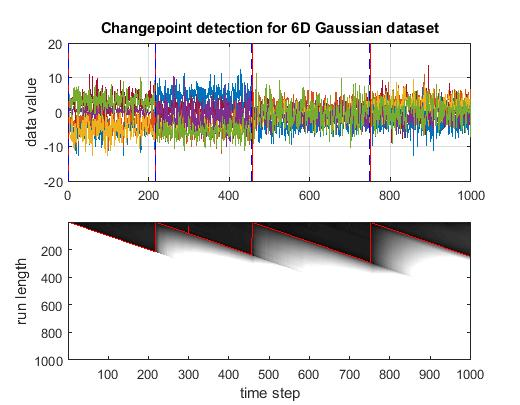
\includegraphics[width=.7\textwidth]{6d_gauss_full.jpg}
\caption{Results of the initial version of the algorithm on a toy dataset with 6 dimensions. In the top plot, dashed blue lines indicate real changepoints and red lines changepoints found by the algorithm. The bottom plot shows posterior probabilities of the run length for each time step, with darker shades indicating higher probability and maxima highlighted in red.}
\label{fig:ex6dims}
\end{figure}

Figure \ref{fig:ex6dims} shows the segmentation of a toy dataset with 6 dimensions and 1000 samples, when using the initial version of the algorithm. From the top plot it can be seen that the location of the changepoints found (shown as vertical red lines) are very close to the real locations of the changepoint (shown as dashed blue lines).

However, the computation increase linearly with each sample, as in fact for each time step $t$ the calculations required increase, because the posterior is calculated $t$ times (for each possible run length starting from the beginning). This results in a longer detection delay for the changepoint when its location is further away from $t=0$, as can be seen in the middle column in Table \ref{tab:delays}.

\begin{table} [h]
\centering
\begin{tabular}{|c|x{4cm}|x{4cm}|}
\hline
\textbf{Changepoint} & \textbf{Detection delay (s) Initial Algorithm} & \textbf{Detection delay (s) Fast Algorithm} \\ \hline
1st & 0 & 0 \\ \hline
2nd & 0.7880 & 0.6063 \\ \hline
3rd & 1.3382 & 0.5193 \\ \hline
4th & 1.6176 & 0.6144 \\ \hline
\end{tabular}
\caption{Time delays of the initial and fast versions of the algorithm to reliably locate changepoints, considering their real temporal location. Delays are stored from simulations in Figure \ref{fig:ex6dims} and Figure \ref{fig:ex6dims_fast}. The first changepoint is at $t=0$ and is known a priori, hence its delay is 0s.}
\label{tab:delays}
\end{table}

However, when considering the bottom plot of Figure \ref{fig:ex6dims}, it was noticed that the run length (indicated by a red line) increases starting from the changepoint and does not go back to higher values, fact that would place the current datum in the previous segment. Moreover, the shade of the posterior probabilities for higher run lengths are very light coloured, marking that the value is very small.

\begin{figure}[h]
\centering
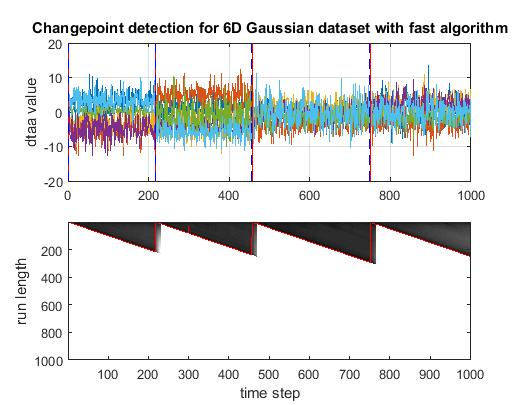
\includegraphics[width=.7\textwidth]{6d_gauss_fast.jpg}
\caption{Results of the "fast" algorithm on the toy dataset with 6 dimensions. In the top plot, dashed blue lines indicate real changepoints and red lines changepoints found by the algorithm. The bottom plot shows posterior probabilities of the run length for each time step, with darker shades indicating higher probability and maxima highlighted in red.}
\label{fig:ex6dims_fast}
\end{figure}

Results of tests with the \textit{fast} version of the algorithm have been shown very positive, as can be seen in Figure \ref{fig:ex6dims_fast}, which is a test performed on the same dataset as in Figure \ref{fig:ex6dims}. The locations of changepoints are found with the same reliability and the detection delays reported in the last column of Table \ref{tab:delays} are much shorter for later changepoints than in the case shown in the middle column. In fact, with the fast version of the algorithm only $t-lastCP$ computations are needed for each time step, where $lastCP$ represents the temporal location of the last changepoint found.

% \begin{table} 
% \centering
% \begin{tabular}{|c|c|}
% \hline
% \textbf{Changepoint} & \textbf{Detection delay (s)} \\ \hline
% 1st & 0 \\ \hline
% 2nd & 0.6063 \\ \hline
% 3rd & 0.5193 \\ \hline
% 4th & 0.6144 \\ \hline
% \end{tabular}
% \caption{Time delay to locate changepoints after first detecting a change for the results in Figure \ref{fig:ex6dims_fast}, using the fast algorithm. The first changepoint is at $t=0$ and is known a priori, hence its detection delay is 0s.}
% \label{tab:delays_fast}
% \end{table}

A second test was then performed to check the difference in time taken to perform the two versions of the detection algorithm on the whole time series. Figure \ref{fig:timeDim} shows the mean and standard deviation over 5 runs of the total time for a time series with 1000 samples and 5 changepoints, with dimensions ranging from 2 to 10. There is a considerable improvement in speed with the "fast" algorithm, especially with higher number of dimensions where it performs almost 4 times faster.\footnote{The actual improvement depend mostly on the number of changepoints and their distance: more frequent changepoints will reduce the total number of computations required, because the run length will never get to a high value.} In both versions, moreover, all changepoints were found close to their original locations, thus proving that there is no loss of reliability with the fast algorithm.

These results demonstrate the strengths of the "fast" algorithm, which was chosen as the only one considered in all later experiments.

\begin{figure} [h]
\centering
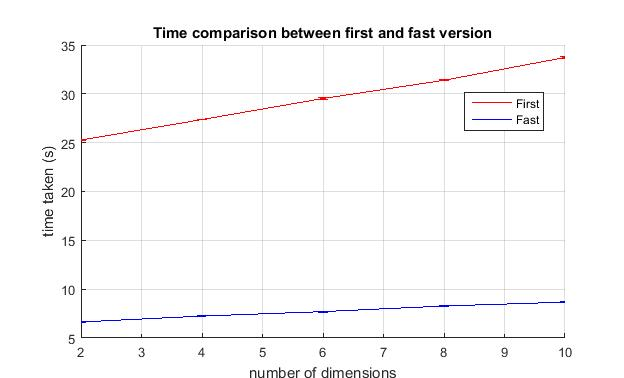
\includegraphics[width=.8\textwidth]{plot_time.jpg}
\caption{Mean and standard deviation of total time to complete the algorithm for the two versions, with a time series with 1000 samples, 5 changepoints and 2-10 dimensions.}
\label{fig:timeDim}
\end{figure}

\section{Experiments on Real Datasets}

After obtaining satisfactory results on toy datasets, the algorithm was then tested on real datasets of two complex sequential tasks: a carrot grating task (as shown in Figure \ref{fig:initial}) and a zucchini peeling task. 

In the case of the carrot grating task, the time series has 7 dimension, the first 3 being the position of the robot's end effector (x, y and z) and the last 4 the orientation quaternions.

Figure \ref{fig:carrot} shows the position of changepoints found, which segment the three tasks (reach, grate and trash) correctly. On the bottom plot of the figure it can be seen that the first changepoint is first detected only after 1000 time steps, although it has occurred about 700 time steps earlier. The detection of the changepoint takes a long time in this case, because the algorithm recognizes there has been a change in the parameters only after the parameters have stabilized in the new segment. On the other hand, thanks to the run length, it is still possible to find the location of the changepoint by subtracting the run length to the current time step.

The segmentation obtained in the end separates the 3 different tasks but does not consider smaller sub-tasks as the ones during the longer "grating" segment in Figure \ref{fig:carrot}. The algorithm, then, appears to be useful as a fast high-level segmentation algorithm.

\begin{figure} [h]
\centering
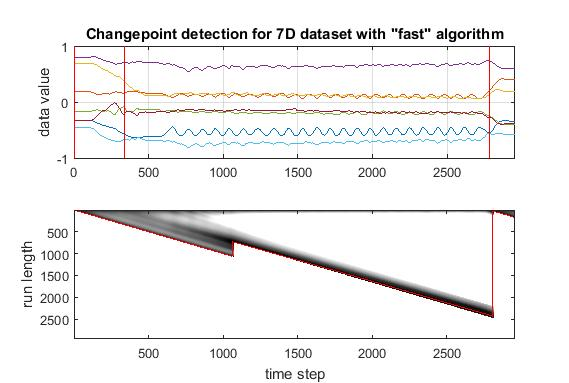
\includegraphics[width=.7\textwidth]{carrot_fast.jpg}
\caption{Results of the Changepoint Detection algorithm on the 7-dimensional carrot grating dataset, with data and changepoints found on the top plot and run length landscape on the bottom.}
\label{fig:carrot}
\end{figure}

The other real datasets that was considered consisted in two 13-dimensional time series of a zucchini peeling task. The first 7 dimension are again the end effector position and orientation in space, while the other 6 dimensions are forces and torques sensed at the end effector.

Results obtained when including all dimensions are visible in Figure \ref{fig:peelAll}, while in Figure \ref{fig:peel7} only the position and orientation dimensions were considered. For both datasets the detection of changepoints in the 13-dimensional time series is very satisfactory, as they are comparable to results obtained from offline batch algorithms on the same datasets which are presented in \cite{lucia} and \cite{nadia}. The main advantage of the proposed online algorithm with respect to the offline ones is that changepoints were recovered by analyzing only one time series online, without the need to wait for many demonstrations of the same task to be completed.

When considering only 7 dimensions as done in Figure \ref{fig:peel7}, changepoints detected delimit segments in the time series at a higher-level of segmentation, similarly to the case in Figure \ref{fig:carrot}. In fact, it can be noticed that the missing forces and torques in the second case are the one which mostly change in the first case, thus determining the other changepoint locations.

The results in the figures reflect the observation which was also made for the carrot grating task, which is the fact that the algorithm seems to segment the data on a higher level. However, this depends also on how the actions are performed. For instance, the top plot tends to group together different peeling motions which are close together in time because the algorithm does not have the time to recognize the change before the next motion starts, while in the bottom plot subsequent motions are generally more separated in time and thus segmented with higher granularity.

This however is not a drawback for the method, as it can be used as prior knowledge on how the task was demonstrated. Also, the segmentation can be used to pre-process the data for further learning algorithms.

\begin{figure} [ht]
\begin{minipage}{\textwidth}
\centering
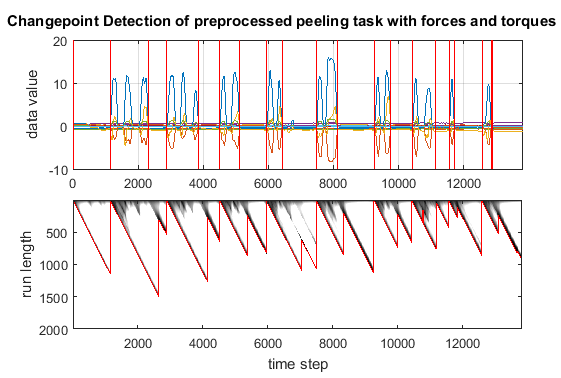
\includegraphics[width=.7\textwidth]{proc1.png}
\end{minipage}
\begin{minipage}{\textwidth}
\centering
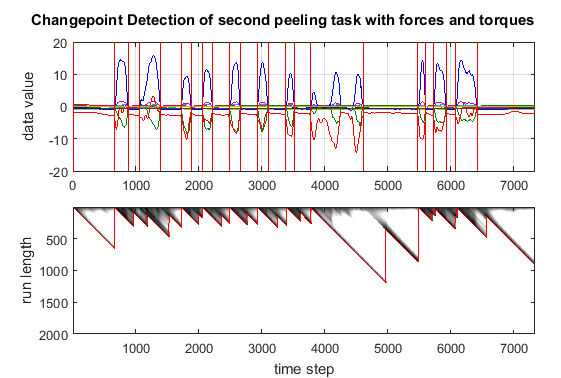
\includegraphics[width=.7\textwidth]{proc2.png}
\end{minipage}
\caption{Results of the Changepoint Detection algorithm on two real datasets of a preprocessed zucchini peeling task. The time series has 13 dimensions: position, orientation quaternions, forces and torques.}
\label{fig:peelAll}
\end{figure}

\begin{figure} [ht]
\begin{minipage}{\textwidth}
\centering
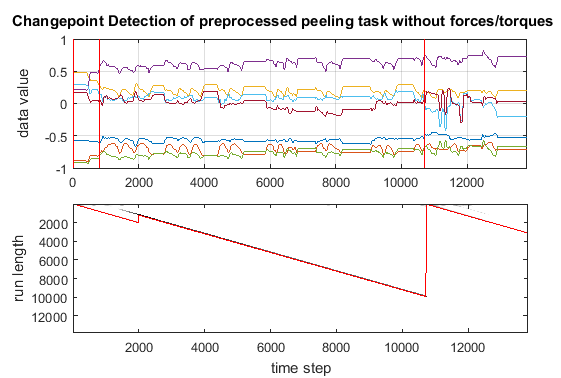
\includegraphics[width=.7\textwidth]{proc1_7dim.png}
\end{minipage}
\begin{minipage}{\textwidth}
\centering
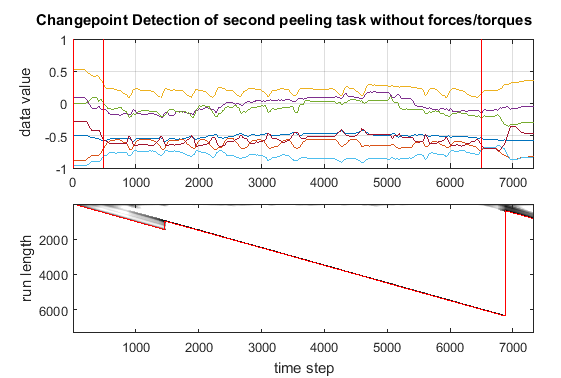
\includegraphics[width=.7\textwidth]{proc2_7dim.png}
\end{minipage}
\caption{Results of the Changepoint Detection algorithm on two real datasets of a preprocessed zucchini peeling task, considering 7 dimensions: position and orientation quaternions.}
\label{fig:peel7}
\end{figure}


\chapter{Conclusion}

In this project we developed a multivariate Bayesian online changepoint detection algorithm and explored approximated solutions for improving the computation time. 

Results show a satisfactory performance in both offline and online datasets.

During the experiments some datasets have not reported successful results, though, as it appeared that a more informative prior on the segment length should have been used. Other types of priors were explored but not considered to keep the algorithm as general as possible, to allow the use in various occasions without the need to set any hyperparameters.

Nonetheless, a further exploration of the topic may be an interesting future step for the project.

Finally, further tests of the real-time implementation should be performed to check the speed performance of the algorithm, and eventually improve it.


\clearpage 
\begin{thebibliography}{9}

\bibitem{lucia}
A. L. Pais et al., \textit{Task Parametrization Using Continuous Constraints Extracted from Human Demonstrations},
IEEE Transactions on Robotics, Vol. 31 (6), pp. 1458 - 1471, 2015

\bibitem{nadia}
N. Figueroa and A. Billard, \textit{Discovering Primitive Motions from Unstructured Heterogeneous Demonstrations},
\url{http://openreview.informatik.uni-freiburg.de/sites/default/files/papers/submission_43.pdf}

\bibitem{adams}
R. Adams and D. Mackay, \textit{Bayesian Online Changepoint Detection},
arXiv:0710.3742 [stat.ML], 2007

\bibitem{fearn1}
P. Fearnhead, \textit{Exact and efficient Bayesian inference for multiple changepoint problems},
Statistics and Computing,
Vol. 16 (2), pp. 203–213, 2006

\bibitem{fearn2}
P. Fearnhead and Z. Liu, \textit{On-line inference for multiple changepoint problems},
Journal of the Royal Statistical Society: Series B (Statistical Methodology), 
Vol. 69 (4), pp. 589–605, 2007

\bibitem{champ}
S. Niekum et al., \textit{CHAMP: Changepoint Detection Using
Approximate Model Parameters},
tech. report CMU-RI-TR-14-10, Robotics Institute, Carnegie Mellon University, 2014

\bibitem{book1}
C. Bishop, \textit{Pattern Recognition and Machine Learning}, Springer, 2006.

\bibitem{book2}
K. Murphy, \textit{Machine Learning: A Probabilistic Perspective}, MIT press, 2012.

\end{thebibliography}

\end{document}